This section presents the main results of the 120 experiments performed as defined in Section \ref{subsec:experimental_design}. The experiments are grouped into subsections according to the measured operation (read or write). In each one of the subsections histograms and tables are present to visualize the results using both metrics (latency expressed in seconds and throughput expressed in rows/second).

Results are reported using the log scale for clarity, as results differing from more than one significant figure are not clearly visible using a histogram representation. Additionally, for each measurement displayed a 95\% confidence interval was also calculated using the bootstrapping technique mentioned in Section \ref{subsec:reliability_validity}. Nonetheless, this interval was not reported in the histograms in this section, as it would be hardly readable as all results are out of each other's 95\% confidence interval. It can still be visioned in the Appendix \todo[inline]{Add ref to appendix} where for each experiment a histogram and a table containing the 95\% confidence interval were reported.

Considering that latency and throughput are inversely correlated (see equation in Section \ref{subsec:eval_process}) trends observed when measuring latency are inversely reflected when data is observed as throughput (e.g. if latency is halved, throughput doubles, if latency quarters, throughput quadruples). This is because all experiments were performed with fixed-size tables.

Due to this correlation between the metrics used, trends will be described using latency (the measured metric), and complemented in brackets for throughput (the computed metric) using an abbreviation (thr:).

\subsection{Writing Experiments}

\begin{figure}
    \centering
    \begin{subfigure}[b]{\textwidth}
        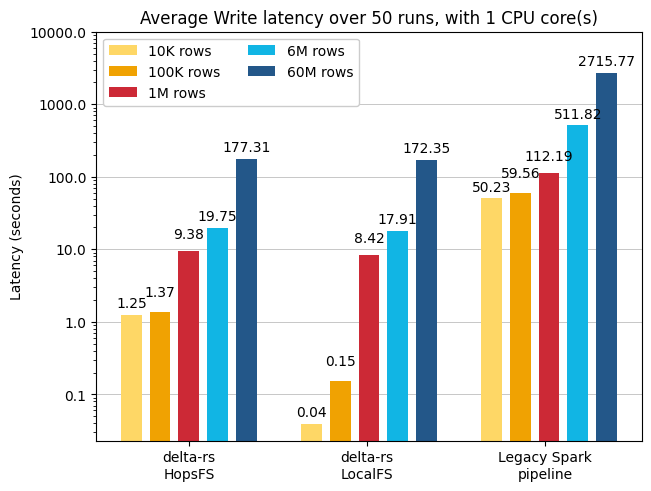
\includegraphics[width=\textwidth]{figures/5-results/write/write_time_1_core.png}
        \caption{Histogram with write latency experiment results}
        \label{fig:res_write_time}
    \end{subfigure}
    
    \begin{subfigure}[b]{\textwidth}
        \begin{tabular}{c c c c c c} 
            \toprule
            Pipeline\Tstrut\Bstrut & \thead{Number\\ of rows} & \thead{1 CPU core latency \\ (seconds)} & \thead{2 CPU cores\\ (\% decrease)} & \thead{4 CPU cores\\ (\% decrease)} & \thead{8 CPU cores\\ (\% decrease)} \\
            \midrule
            \multirow{5}{4em}{delta-rs\\ HopsFS} & 10K & 1.250881458553 & -0.92 & 2.75 & -9.33\\ 
            & 100K & 1.368281275251 & 4.40 & 2.34 & 5.54\\ 
            & 1M &   9.381529912744 & 9.23 & 10.32 & 11.52\\
            & 6M &   19.75469028131 & 17.54 & 17.87 & 20.33\\
            & 60M &  177.3070700216 & 24.39 & 30.01 & 31.22\\
            \midrule
            \multirow{5}{4em}{delta-rs\\ LocalFS} & 10K & 0.039575374951 & -21.88 & -15.53 & -11.25\\ 
            & 100K & 0.152402458205 & 10.01 & 13.54 & 10.45\\ 
            & 1M &   8.422528293415 & 14.69 & 14.68 & 14.17\\
            & 6M &   17.90634508900 & 14.74 & 18.71 & 20.24\\
            & 60M &  172.3455279090 & 24.67 & 29.57 & 30.38\\
            \midrule
            \multirow{5}{4em}{Legacy \\ Spark} & 10K & 50.22767340044 & -0.99 & -2.10 & -1.99\\ 
            & 100K & 59.56187132072 & -0.38 & 0.06 & -1.20\\ 
            & 1M &   112.1904872782 & 3.23 & 3.01 & 2.50\\
            & 6M &   511.8169330835 & 7.51 & 5.83 & 7.01\\
            & 60M &  2715.772857148 & 13.81 & 13.61 & 14.39\\
            \bottomrule
        \end{tabular}
        \caption{Table containing the write latency experiment results compared across multiple \glstext{CPU} configurations}
        \label{tbl:res_write_time_cpu_perc}
    \end{subfigure}
    \caption{Histogram (a) and Table (b) reporting the write latency experiment results also across different \glstext{CPU} configurations}
    \label{fig_tbl:res_write_time}
\end{figure}

\begin{figure}
    \centering
    \begin{subfigure}[b]{\textwidth}
        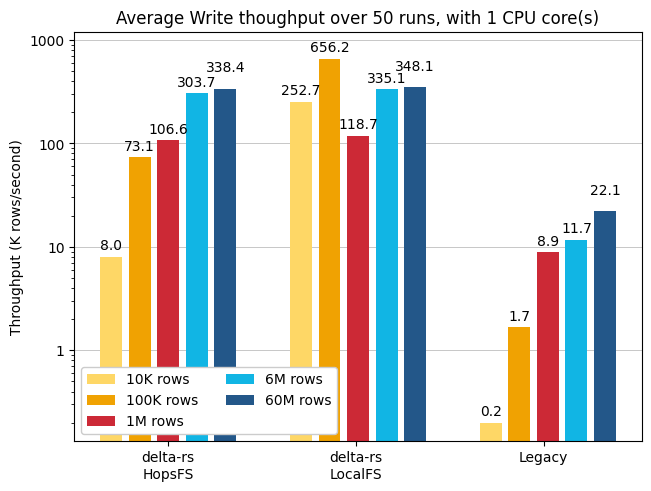
\includegraphics[width=\textwidth]{figures/5-results/write/write_throughput_1_core.png}
        \caption{Histogram with write throughput experiment results}
        \label{fig:res_write_throughput}
    \end{subfigure}
    
    \begin{subfigure}[b]{\textwidth}
        \begin{tabular}{c c c c c c} 
            \toprule
            Pipeline\Tstrut\Bstrut & \thead{Number\\ of rows} & \thead{1 CPU core throughput \\ (k rows/second)} & \thead{2 CPU cores\\ (\% increase)} & \thead{4 CPU cores\\ (\% increase)} & \thead{8 CPU cores\\ (\% increase)} \\
            \midrule
            \multirow{5}{4em}{delta-rs\\ HopsFS} & 10K & 7.994362640538 & -0.91 & 2.83 & -8.53\\ 
            & 100K & 73.08438828236 & 4.60 & 2.40 & 5.87\\ 
            & 1M &   106.5924224834 & 10.17 & 11.51 & 13.01\\
            & 6M &   303.7253388718 & 21.27 & 21.76 & 25.52\\
            & 60M &  338.3959815741 & 32.26 & 42.87 & 45.39\\
            \midrule
            \multirow{5}{4em}{delta-rs\\ LocalFS} & 10K & 252.6823817158 & -17.95 & -13.44 & -10.12\\ 
            & 100K & 656.1573952099 & 11.13 & 15.66 & 11.67\\ 
            & 1M &   118.7291945082 & 17.22 & 17.21 & 16.51\\
            & 6M &   335.0767546463 & 17.29 & 23.02 & 25.38\\
            & 60M &  348.1378410449 & 32.76 & 41.99 & 43.65\\
            \midrule
            \multirow{5}{4em}{Legacy \\ Spark} & 10K & 0.199093434415 & -0.98 & -2.06 & -1.95\\ 
            & 100K & 1.678926430325 & -0.38 & 0.06 & -1.19\\ 
            & 1M &   8.913411682753 & 3.34 & 3.10 & 2.57\\
            & 6M &   11.72294156790 & 8.12 & 6.19 & 7.54\\
            & 60M &  22.09315843262 & 16.02 & 15.76 & 16.81\\
            \bottomrule
        \end{tabular}
        \caption{Table containing the write throughput experiment results compared across multiple \glstext{CPU} configurations}
        \label{tbl:res_write_throughput_cpu_perc}
    \end{subfigure}
    \caption{Histogram (a) and Table (b) reporting the write throughput experiment results also across different \glstext{CPU} configurations}
    \label{fig_tbl:res_write_throughput}
\end{figure}

Figure \ref{fig_tbl:res_write_time} and Figure \ref{fig_tbl:res_write_throughput} show the write latency and throughput respectively of the write operations performed on three different systems defined in Section \ref{subsec:experimental_design} when writing the five different tables defined in Section \ref{subsec:dataset}. Both histograms, i.e. Figures \ref{fig:res_write_time} and \ref{fig:res_write_throughput}, report the data from the 1 \gls{CPU} core experiment while the tables, i.e. Figures \ref{tbl:res_write_time_cpu_perc} and \ref{tbl:res_write_throughput_cpu_perc}, report both the 1 \gls{CPU} core experiment data and also a calculated percentage of improvement (decrease in the case of latency, increase in the case of throughput) of the specified metric as the \gls{CPU} cores increase.

\subsubsection*{delta-rs on \glsentryshort{HopsFS} vs. delta-rs on \glsentryshort{LocalFS}}

The latency (thr: throughput) measured using the delta-rs on \gls{LocalFS} pipeline results around ten times lower (thr: higher) than the latency (thr: throughput) measured using the delta-rs on \gls{HopsFS} pipeline for small tables (10K and 100K rows). On the other hand, the latency (thr: throughput) in the two pipelines is more similar (same significant figure) on experiments performed with larger tables (1M, 10M, 6M, and 60M rows). Overall the latency (thr: throughput) measured in the delta-rs on \gls{LocalFS} pipeline remains lower (thr: higher) in absolute terms than the latency (thr: throughput) measured using the delta-rs on \gls{HopsFS} pipeline in all experiments.

\subsubsection*{delta-rs on \glsentryshort{HopsFS} vs. Legacy Spark pipeline}

The latency (thr: throughput) measured using the delta-rs on \gls{HopsFS} pipeline results more than ten times lower (thr: higher) than the latency (thr: throughput) measured using the Legacy Spark pipeline in all experiments. This trend results more prominent for smaller tables (10K and 100K rows) where latency (thr: throughput) measured using the delta-rs on \gls{HopsFS} pipeline is forty times lower (thr: higher) than the latency measured using the Legacy Spark pipeline. While the tendency is less marked for larger tables (6M and 60M rows) where latency (thr: throughput) measured using the delta-rs on \gls{HopsFS} pipeline is around twenty times lower (thr: higher) than the latency (thr: throughput) measured using the Legacy Spark pipeline.

\subsubsection*{Change of performance as the \glsentryshort{CPU} cores increase}

During experiments with more \gls{CPU} cores, in delta-rs based pipelines (writing on \gls{HopsFS} or \gls{LocalFS}) the latency (thr: throughput) during write operation decreases (thr: increases) by a considerable amount: 20-30\% (thr: 30-40\%), only when writing larger tables (6M and 60M rows), while it decreases (thr: increases) by a lower margin: 5-10\% (thr: 5-15\%) on smaller tables (100K and 1M rows), even slightly increasing (thr: decreasing) on the smallest table (10K rows). It should be noted that latency (thr: throughput) decreases (thr: increases) as described in the 2 \gls{CPU} cores experiments, remaining on similar improvements even with more \gls{CPU} cores.

Considering the Legacy Spark pipeline, experiments with more \gls{CPU} cores did not decrease (thr: increase) the latency (thr: throughput) by more than 7\% (thr: 8\%) except for the largest table (60M rows). This table benefitted from a latency (thr: throughput) decrease (the: increase) of around 14\% (thr: 16\%). The smallest tables (10K and 100K) even reported slight increases (thr: decreases) in the latency measured.

\subsection{Reading Experiments}

\begin{figure}
    \centering
    \begin{subfigure}[b]{\textwidth}
        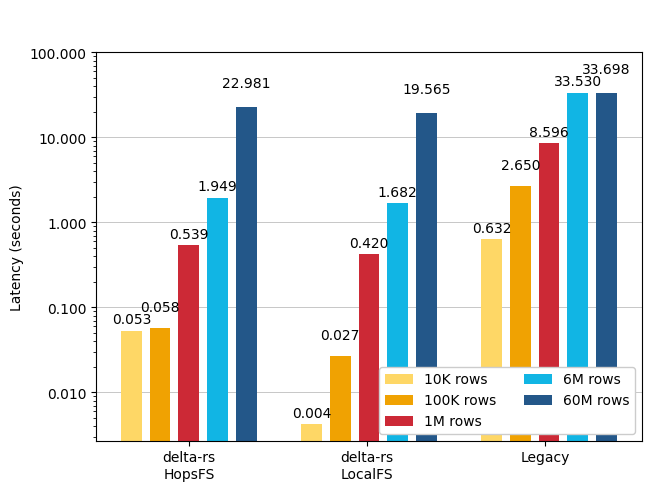
\includegraphics[width=\textwidth]{figures/5-results/read/read_time_1_core.png}
        \caption{Histogram with read latency experiment results}
        \label{fig:res_read_time}
    \end{subfigure}
    
    \begin{subfigure}[b]{\textwidth}
        \begin{tabular}{c c c c c c} 
            \toprule
            Pipeline\Tstrut\Bstrut & \thead{Number\\ of rows} & \thead{1 CPU core latency \\ (seconds)} & \thead{2 CPU cores\\ (\% decrease)} & \thead{4 CPU cores\\ (\% decrease)} & \thead{8 CPU cores\\ (\% decrease)} \\
            \midrule
            \multirow{5}{4em}{delta-rs\\ HopsFS} & 10K & 0.053427784961 & 22.65 & 18.84 & 18.95\\ 
            & 100K & 0.057573573334 & 1.15 & 3.76 & 5.19\\ 
            & 1M & 0.538551778791 & 56.53 & 65.00 & 67.71\\
            & 6M & 1.948992908833 & 53.40 & 72.74 & 74.48\\
            & 60M & 22.98065653875 & 50.34 & 75.72 & 87.20\\
            \midrule
            \multirow{5}{4em}{delta-rs\\ LocalFS} & 10K & 0.004193598319 & 31.48 & 35.91 & 29.66\\ 
            & 100K & 0.026966840860 & 51.54 & 65.76 & 64.84\\ 
            & 1M &   0.420096789910 & 52.45 & 78.64 & 89.75\\
            & 6M &   1.682239274377 & 55.56 & 77.99 & 89.57\\
            & 60M &  19.56547400704 & 51.72 & 75.41 & 88.32\\
            \midrule
            \multirow{5}{4em}{Legacy \\ Spark} & 10K & 0.631598152258 & 1.06 & -0.67 & 0.67\\ 
            & 100K & 2.650107346201 & -0.50 & 0.39 & -0.46\\ 
            & 1M &   8.596367535570 & -0.24 & -1.81 & 2.89\\
            & 6M &   33.52964549822 & 0.46 & 0.23 & 0.30\\
            & 60M &  33.69772492026 & 0.16 & 0.13 & 1.64\\
            \bottomrule
        \end{tabular}
        \caption{Table containing the read latency experiment results compared across multiple \glstext{CPU} configurations}
        \label{tbl:res_read_time_cpu_perc}
    \end{subfigure}
    \caption{Histogram (a) and Table (b) reporting the read latency experiment results also across different \glstext{CPU} configurations}
    \label{fig_tbl:res_read_time}
\end{figure}

\begin{figure}
    \centering
    \begin{subfigure}[b]{\textwidth}
        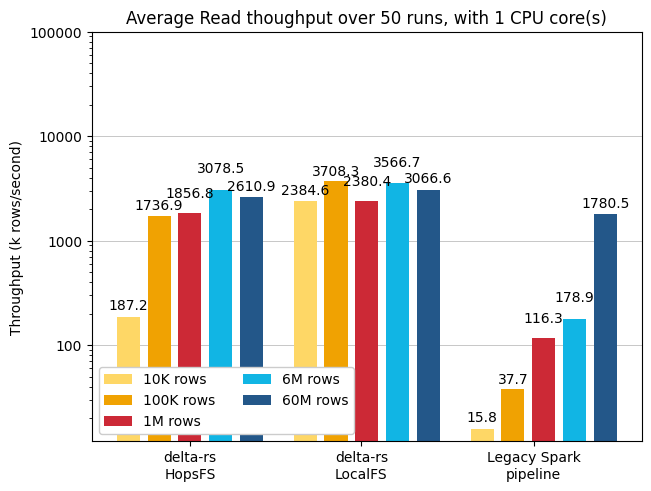
\includegraphics[width=\textwidth]{figures/5-results/read/read_throughput_1_core.png}
        \caption{Histogram with read throughput experiment results}
        \label{fig:res_read_throughput}
    \end{subfigure}
    
    \begin{subfigure}[b]{\textwidth}
        \begin{tabular}{c c c c c c} 
            \toprule
            Pipeline\Tstrut\Bstrut & \thead{Number\\ of rows} & \thead{1 CPU core throughput \\ (k rows/second)} & \thead{2 CPU cores\\ (\% increase)} & \thead{4 CPU cores\\ (\% increase)} & \thead{8 CPU cores\\ (\% increase)} \\
            \midrule
            \multirow{5}{4em}{delta-rs\\ HopsFS} & 10K & 187.1685305156 & 29.28 & 23.21 & 23.38\\ 
            & 100K & 1736.907998044 & 1.17 & 3.90 & 5.48\\ 
            & 1M &   1856.831672237 & 130.02 & 185.74 & 209.69\\
            & 6M &   3078.512996536 & 114.57 & 266.87 & 291.92\\
            & 60M &  2610.891464254 & 101.35 & 311.83 & 681.03\\
            \midrule
            \multirow{5}{4em}{delta-rs\\ LocalFS} & 10K & 2384.586991466 & 45.94 & 56.04 & 42.18\\ 
            & 100K & 3708.257875522 & 106.37 & 192.07 & 184.38\\ 
            & 1M &   2380.403811732 & 110.28 & 368.24 & 875.15\\
            & 6M &   3566.674545879 & 125.01 & 354.40 & 858.64\\
            & 60M &  3066.626445053 & 107.11 & 306.75 & 756.07\\
            \midrule
            \multirow{5}{4em}{Legacy \\ Spark} & 10K & 15.83285189203 & 1.07 & -0.67 & 0.67\\ 
            & 100K & 37.73432051472 & -0.50 & 0.39 & -0.45\\ 
            & 1M &   116.3282044261 & -0.24 & -1.78 & 2.98\\
            & 6M &   178.9461209876 & 0.46 & 0.23 & 0.30\\
            & 60M &  1780.535633843 & 0.16 & 0.13 & 1.67\\
            \bottomrule
        \end{tabular}
        \caption{Table containing the read throughput experiment results compared across multiple \glstext{CPU} configurations}
        \label{tbl:res_read_throughput_cpu_perc}
    \end{subfigure}
    \caption{Histogram (a) and Table (b) reporting the read throughput experiment results also across different \glstext{CPU} configurations}
    \label{fig_tbl:res_read_throughput}
\end{figure}

Figure \ref{fig_tbl:res_read_time} and Figure \ref{fig_tbl:res_read_throughput} show the read latency and throughput respectively of the read operations performed on three different systems defined in Section \ref{subsec:experimental_design} when reading the five different tables defined in Section \ref{subsec:dataset}. Both histograms, i.e. Figures \ref{fig:res_read_time} and \ref{fig:res_read_throughput}, report the data from the 1 \gls{CPU} core experiment while the tables, i.e. Figures \ref{tbl:res_read_time_cpu_perc} and \ref{tbl:res_read_throughput_cpu_perc}, report both the 1 \gls{CPU} core experiment data and also a calculated percentage of improvement (decrease in the case of latency, increase in the case of throughput) of the specified metric as the \gls{CPU} cores increase.

\subsubsection*{delta-rs on \glsentryshort{HopsFS} vs. delta-rs on \glsentryshort{LocalFS}}

The latency (thr: throughput) measured using the delta-rs on \gls{LocalFS} pipeline results around ten times lower (thr: higher) than the latency (thr: throughput) measured using the delta-rs on \gls{HopsFS} pipeline in the experiment with the smallest table (10K rows). On the other hand, the latency (thr: throughput) in the two pipelines is more similar (same significant figure) on experiments performed with larger tables (100K, 1M, 10M, 6M, and 60M rows). Overall the latency (thr: throughput) measured in the delta-rs on \gls{LocalFS} pipeline remains lower (thr: higher) in absolute terms than the latency (thr: throughput) measured using the delta-rs on \gls{HopsFS} pipeline in all experiments.

\subsubsection*{delta-rs on \glsentryshort{HopsFS} vs. Legacy Spark pipeline}

The latency (thr: throughput) measured using the delta-rs on \gls{HopsFS} pipeline results more than ten times lower (thr: higher) than the latency (thr: throughput) measured using the Legacy Spark pipeline in all but the experiment with the largest table (60M rows), where the latency (thr: throughput)of the first pipeline is only 47\% lower (thr: higher) than the second. 

\subsubsection*{Change of performance as the \glsentryshort{CPU} cores increase}

During experiments with more \gls{CPU} cores, in delta-rs based pipelines (reading on \gls{HopsFS} or \gls{LocalFS}) the latency (thr: throughput) during read operation decreases (thr: increases) by a considerable amount: +50\% (thr: +100\%), when reading larger tables (1M, 6M and 60M rows), while it decreases (thr: increases) by a lower margin: 20-30\% (thr: 30-45\%) on smaller tables (10K and 100K rows). It should be noted that latency decreases (thr: increases) in reads with larger tables (1M, 6M, and 60M rows) following an inverse linear relationship with the increase of \gls{CPU} cores: 2 \gls{CPU} cores, latency halves, 4 \gls{CPU} cores, latency quarters, 8 \gls{CPU} cores, latency is decreased to an eighth. On the other hand, throughput follows a linear relationship with the increase of \gls{CPU} cores.

Considering the Legacy Spark pipeline, experiments with more \gls{CPU} cores did not decrease (thr: increase) the latency (thr: throughput) by more than 2\% (thr: 8\%). Histograms comparing the three pipelines, look radically different in experiments with more \gls{CPU} cores, due to how delta-rs scales with the increase of \gls{CPU} cores. They can be accessed in the Appendix \todo[inline]{Add ref. to appendix}.

\subsection{Legacy Spark pipeline write latency breakdown}

\begin{figure}
    \centering
    \begin{subfigure}[b]{\textwidth}
        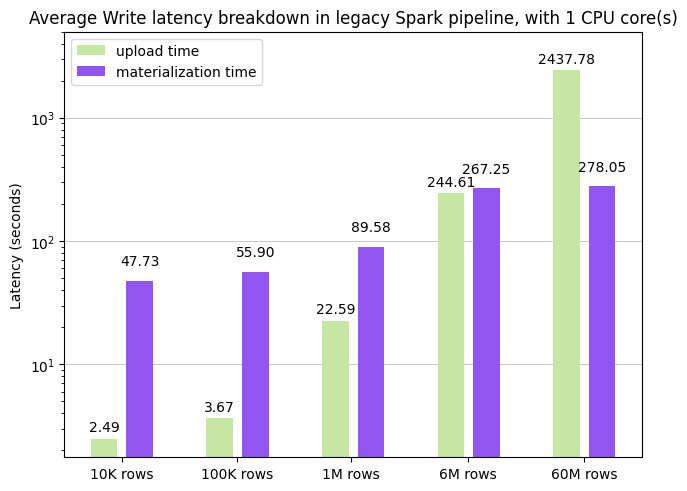
\includegraphics[width=\textwidth]{figures/5-results/hudi_virtualiz_1_core.png}
        \caption{Histogram displaying the contributions to the write latency of the upload and materialization steps in the legacy Spark pipeline}
        \label{fig:hudi_virtualiz_breakdown}
    \end{subfigure}
    
    \begin{subfigure}[b]{\textwidth}
        \begin{tabular}{c c c c c c c c c} 
            \toprule
            \multirow{2}{*}{\thead{Number\\ of rows}} & \multicolumn{2}{c}{\thead{1 CPU core\\ latency (seconds)}} & \multicolumn{2}{c}{\thead{2 CPU cores\\ (\% decrease)}} & \multicolumn{2}{c}{\thead{4 CPU cores\\ (\% decrease)}} & \multicolumn{2}{c}{\thead{8 CPU cores\\ (\% decrease)}}\\
            & upl. & mat. & upl. & mat. & upl. & mat. & upl. & mat.\\
            \midrule
            10K &  2.48653 & 47.726 & 3.99 & -1.27 & 4.10 & -2.47 & 4.22 & -2.35\\
            100K & 3.66844 & 55.900 & 6.37 & -0.78 & 5.55 & -0.27 & 6.25 & -1.69\\
            1M   & 22.5934 & 89.575 & 17.52 & -0.39 & 14.89 & -0.01 & 16.51 & -1.05\\
            6M   & 244.612 & 267.24 & 15.83 & -0.10 & 13.46 & -1.15 & 15.10 & -0.38\\
            60M &  2437.78 & 278.05 & 15.33 & 0.39 & 15.15 & 0.16 & 15.94 & 0.82\\
            \bottomrule
        \end{tabular}
        \caption{Table showing the contributions to the write latency of the upload and materialization steps in the legacy Spark pipeline and its change at different \glstext{CPU} configurations}
        \label{tbl:hudi_virtualiz_breakdown_cpu_perc}
    \end{subfigure}
    \caption{Histogram (a) and Table (b) reporting the contributions to the write latency of the upload and materialization steps in the legacy Spark pipeline and it changes at different \glstext{CPU} configurations}
    \label{fig_tbl:hudi_virtualiz_breakdown}
\end{figure}

Figure \ref{fig_tbl:hudi_virtualiz_breakdown} shows the write latency breakdown of the Legacy Spark pipeline into upload time and materialization time, the different steps of the Legacy Spark pipeline as explained in Section \todo[inline]{Insert ref. to upload materialization expl.}. The breakdown is proposed for all the five different tables defined in Section \ref{subsec:dataset}. Figure \ref{fig:hudi_virtualiz_breakdown} reports the data from the 1 \gls{CPU} core experiment while Figure \ref{tbl:hudi_virtualiz_breakdown_cpu_perc} reports both the 1 \gls{CPU} core experiment data and also a calculated percentage of improvement (decrease) of the latency as the \gls{CPU} cores increase.

Considering the upload time contribution to the write latency, this represents a small percentage (around 5\%) when writing smaller tables (10K and 100K rows), while its contribution grows following a similarly linear pattern in larger tables (between 100K and 60M rows). This changes radically the proportion between the upload and materialized contribution to the write latency, making the upload time 90\% of the total write latency for the 60M rows table. On the other hand, the materialization time contribution while starting with high latency contribution (95\% of the total), its absolute value does not increase by a considerable amount (less than a significant figure) even if the table size increased by three significant figures.

Observing the results of experiments using more \gls{CPU} cores, the upload time benefits from a higher number of \gls{CPU} cores in particular with larger tables (15\% latency decrease) and less with smaller tables (4\% latency decrease). On the other hand, the materialize time does not improve performance having either small decreases in latency or small increases (both around 1-2\%).

\subsection{In-memory resources usage}
\label{subsec:resources_usage}

The experimental environment resources defined in Section \ref{subsec:exp_env} were adjusted according to the computational needs. In particular, write operations were demanding on the available \gls{RAM} resources, requiring up to 24 GBs to operate with the larger tables (6M and 60M rows). The system was adjusted to allocate 32768 MB of \gls{RAM}, so it could avoid slowing down operations.